%%%%%%%%%%%%%%%%%%%%%%%%%%%%%%%%%%%%%%%%%%%%%%%%%%%%%%%%%%
% Tau LaTeX Class
% Trading Bot Thesis Example (with Orderbook image)
%%%%%%%%%%%%%%%%%%%%%%%%%%%%%%%%%%%%%%%%%%%%%%%%%%%%%%%%%%
\documentclass[9pt,a4paper,twocolumn,twoside]{tau-class/tau}
\usepackage[english]{babel}
\usepackage{float}  % for [H] if needed
\usepackage{subcaption} % only if you're using sub-figures

%----------------------------------------------------------
% TITLE
%----------------------------------------------------------
\title{Automated Trading Bot: Feinkonzept}

%----------------------------------------------------------
% AUTHORS, AFFILIATIONS AND PROFESSOR
%----------------------------------------------------------
\author[a,1]{Juri Stoffers}
\affil[a]{Gymthun}
\professor{Begleitperson: Dr. Ostrin Geoffrey}

%----------------------------------------------------------
% FOOTER INFORMATION
%----------------------------------------------------------
\footinfo{Matura Project}
\theday{April 2025}
\leadauthor{S.}

%----------------------------------------------------------
% If you remove or comment out this entire block, the abstract is gone:
% \begin{abstract}
% Here was the abstract text
% \end{abstract}

% If you remove or comment out \keywords, that also disappears:
% \keywords{Trading Bot, Backtesting, System Design, Automated Trading}

%----------------------------------------------------------
\begin{document}

\maketitle
\thispagestyle{firststyle}

% \tableofcontents
% \linenumbers

%----------------------------------------------------------
\section{Define My Goals \& Requirements}

\taustart{} I start by deciding what kind of trading I want to pursue—momentum, 
arbitrage, or another strategy. I set clear targets for profits and acceptable 
losses, and choose the markets I'll focus on (crypto, stocks, or forex). 
I also consider performance requirements like speed, reliability, and 
implementation complexity.

%----------------------------------------------------------
\section{Outline My System Design}

\subsection{Data Sources}
I gather both real-time and historical market data to feed my bot, ensuring 
I have enough coverage for backtesting and live operations.



\subsection{Signal Processing}
I develop modules to analyze data for trade signals, whether it's technical 
indicators (e.g., EMA, Orderbook Delta) or more advanced methods (machine learning). 





\subsection{Order Management}
I connect to broker APIs so my bot can execute trades automatically. This 
includes handling order placement, cancellation, and partial fills.

\subsection{Risk Management}
Safety features like stop-loss orders and position sizing help me control 
potential drawdowns. I might use trailing stops or percentage-based 
position sizing.

\subsection{Monitoring}
I set up real-time tracking and logging to catch issues before they escalate, 
and to log trades for auditing performance over time.

%----------------------------------------------------------
\section{Backtesting \& Simulation}

Before going live, I test my strategy on historical data to refine it and 
uncover potential flaws. I also run a simulated (paper-trading) environment 
to confirm the bot’s logic and that my strategy doesn't suffer from overfit without risking real funds. My plan is to test more than one strategy in the live test with paper money in case my main strategy doesn't work at all.

\subsection{Performance Thresholds}
To avoid misleading results, I apply realistic performance expetations and compare my strategy to a random buy sell strategy.
A sharpen ratio below 1.5 is considered as realistic for short- to mid-term strategies in volatile markets like crypto.
A draw down above 30 percent is considered critical and requires either risk adjustments or moving on to another strategy. 

%----------------------------------------------------------
\section{Implementation \& Operation}

I choose a programming language (e.g., Python) for its extensive libraries 
and community support. I build the system in modular parts so I can update 
individual sections without overhauling the entire setup. Finally, I 
integrate security measures like API encryption and strict access 
controls, while staying aware of regulatory requirements.

\noindent
This plan covers key areas: strategy, system design, testing, and secure 
live operation, giving me a roadmap for a trading bot that could potentially 
be profitable in real markets.

%----------------------------------------------------------
\section{Feinkonzept Notes (Additional Topics)}

\subsection{Data Creation}
\begin{itemize}
  \item Data sources
  \item Creating a good timeseries dataset
  \item Hosting data creation process
  \item External datasources for out-of-sample testing
\end{itemize}


\subsection{What is Bitcoin}
A form of digital currency that uses blockchain technology to support transactions between users on a decentralized network.

\subsection{How is the Price of Bitcoin Determined (Auction Principle)}

Below is an example “orderbook” image illustrating how bids and asks are 
arranged in the marketplace:

\begin{figure}[H]
    \centering
    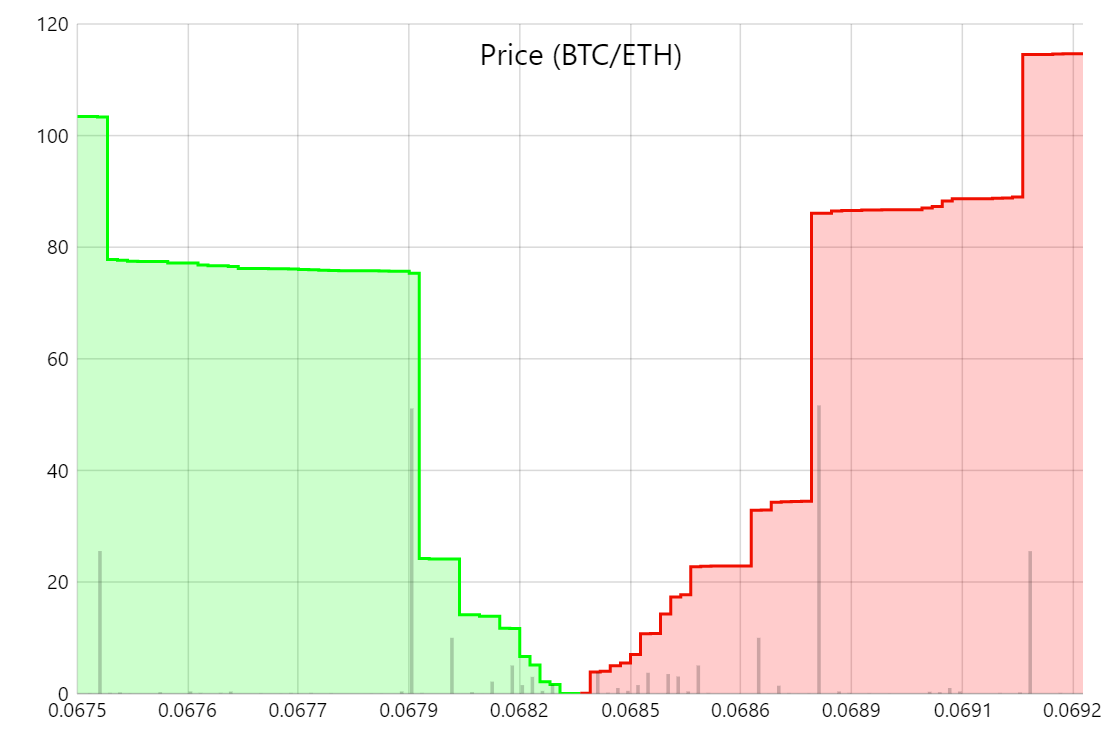
\includegraphics[width=0.85\columnwidth]{figures/orderbook.png}
    \caption{Example orderbook visualization, showing bid/ask levels.}
    \label{fig:orderbook}
\end{figure}

\subsection{Backtesting Details}
\begin{itemize}
  \item Testing different kinds of strategies (Sample vs Out-of-sample)
  \item Sharpe ratio threshold (e.g., below 1.5 = more realistic)
  \item Real-time paper trading test
  \item Outline which indicators I’ll be using
\end{itemize}

\section{Efficient Market Hypothesis}

Is it possible to abstract money from the market? The \textbf{EMH} states that markets fully price in all information, making it impossible to beat the market.

\begin{itemize}
    \item Market have \textbf{temporary inefficiens}, the goal is to exploit those before they go away. Especiallly with in the crypto market where a lot of margin calls occure (forced sells/buys)
    \item Simple moving average cross over strategies might be widely known, there might be more \textbf{complex stratgies} (hiden edge)
    \item \textbf{Behavioral Factors} also play a big role, the Efficient Market Hypothesis assumes rational players, yet many traders execute based on emotions biases. A disciplined can exploit this behavioral inefficiencie.
\end{itemize}





%----------------------------------------------------------
\end{document}
